\documentclass[a4paper,12pt]{article}

\usepackage{amsmath}
%\usepackage{cite}
\usepackage[hidelinks]{hyperref}
\usepackage{geometry}
\usepackage{subcaption}
\usepackage{graphicx}
\usepackage{booktabs} 
\usepackage{multirow}
\usepackage{siunitx}
\usepackage{natbib}
\usepackage{url}
\usepackage[english]{babel}
\usepackage{blindtext}
\usepackage{amsmath}
\usepackage{algorithm}
\usepackage[noend]{algpseudocode}




\makeatletter
\def\BState{\State\hskip-\ALG@thistlm}
\makeatother


\usepackage{fancyhdr}
\pagestyle{fancy}
\rhead{}

\geometry{left=30mm,right=30mm,top=35mm,bottom=30mm,headheight=15pt}

\graphicspath{{./img/}}


\begin{document}
	
	\begin{titlepage}
		\centering
		\begin{figure}[!h]
			\centering
			
\includegraphics[width=0.5\textwidth]{UZH}
		\end{figure}
		\Large{\textbf{example}\\}

		
		\vfill 
		
		\large{Filip Sprusansky \\ 
				second name \\}
		
		\vfill
			
		\large{November 15, 2020}
		
		\vfill
		\vfill
	
		\large{Digital Tools for Finance \\prof 1 \& prof 2 \\ }
	
		\vfill
		\begin{abstract}
		\noindent
			\blindtext
			
			\vspace{3mm}
			
			\textbf{Keywords:} .
		\end{abstract}
		
		
	\end{titlepage}
	
	%\clearpage\thispagestyle{empty}\addtocounter{page}{-1}\mbox{}\clearpage
	
	\clearpage
	\tableofcontents
	
	\clearpage
	\listoffigures
	
	\clearpage
	\listoftables
	\clearpage	
	
	\section{Section 1}
	\subsection{Subsection 1}
    \blindtext
    \subsection{Subsection 2}
    \blindtext
    \begin{itemize}
    	\item Item 1
    	\item Item 2
    	\begin{itemize}
    		\item Subitem 1
    		\item Subitem 2
    	\end{itemize}
    	\item Item 3
    \end{itemize}
    \section{Section 2}
    \subsection{Subsection 1}
    \blindtext
    \begin{enumerate}
    	\item Item 1
    	\item Item 2
    	\begin{enumerate}
    		\item Subitem 1
    		\item Subitem 2
    	\end{enumerate}
    	\item Item 3
    \end{enumerate}
    Aligned system of equations with numbers and labels:
	\begin{align}
		y &= 2 + x \label{eq1} \\
		x &= y + 7 + z \label{eq2}
	\end{align}
	Reference equation 1 (\ref{eq1}) and equation 2 (\ref{eq2}). Next is system of equations with one number:
	\begin{equation}
	\begin{aligned}
		y &= 2 + x  \\
		x &= y + 7 + z
	\end{aligned}
	\label{eq3}
	\end{equation}
	
	Reference system (\ref{eq3}). System with some numbers:
	\begin{align}
		y &= 2 + x  \nonumber \\
		x &= y + 7 + z \\
		y &= 2 + x  \nonumber \\
		x &= y + 7 + z 
	\end{align}
	\section{Section 3}
	\subsection{Subsection 1}
	Now some tables with caption. Source of this table is project for another class.
	\begin{table}[H]
	\begin{center}
    \begin{tabular}{l l l l l l l}
    \toprule
    \multicolumn{7}{c}{Moreira Muir Strategy Results starting 1946} \\
    \midrule
             Statistic &     Mkt$^{\sigma}$ &     SMB$^{\sigma}$ &    HML$^{\sigma}$ &     Mkt &    SMB &     HML \\
    \midrule
  Avg Total Return &    0.83 &    0.24 &    0.57 &    0.86 &   0.35 &    0.62 \\
 Avg Excess Return &    0.51 &   -0.09 &    0.25 &    0.53 &   0.03 &    0.29 \\
 Std Excess Return &    4.25 &     2.8 &    2.65 &    4.25 &   2.81 &    2.65 \\
  Sharpe Geometric &    0.41 &   -0.11 &    0.32 &    0.44 &   0.03 &    0.38 \\
          Skewness &    0.17 &   -0.98 &     0.3 &   -0.54 &    0.5 &    0.45 \\
          Kurtosis &    5.48 &     9.6 &    5.07 &    1.79 &   6.61 &    2.92 \\
               Min &  -20.19 &  -20.73 &  -15.38 &  -23.25 &  -15.6 &  -11.39 \\
               Max &   28.08 &   15.96 &   16.24 &   16.16 &  22.19 &   14.28 \\
             alpha &    1.97 &    -1.1 &    0.68 &    -0.0 &   -0.0 &    -0.0 \\
       Factor Beta &    0.69 &    0.68 &    0.69 &     1.0 &    1.0 &     1.0 \\
               PSR &    0.27 &     0.0 &    0.04 &     0.5 &    0.5 &     0.5 \\
    \bottomrule
    \end{tabular}
	 \caption[Moreira Muir Strategy Results]{Table shows the results from the orignial strategy presented by \cite{Moreira2017}. "$Factor^{\sigma}$" denotes the vol timed strategies.}
    \label{tab:MMresults}
    \end{center}
    \end{table}
	Reference the table: Table \ref{tab:MMresults}\\
	
	Now lets try some figures:
		\begin{figure}[H]
			\centering
			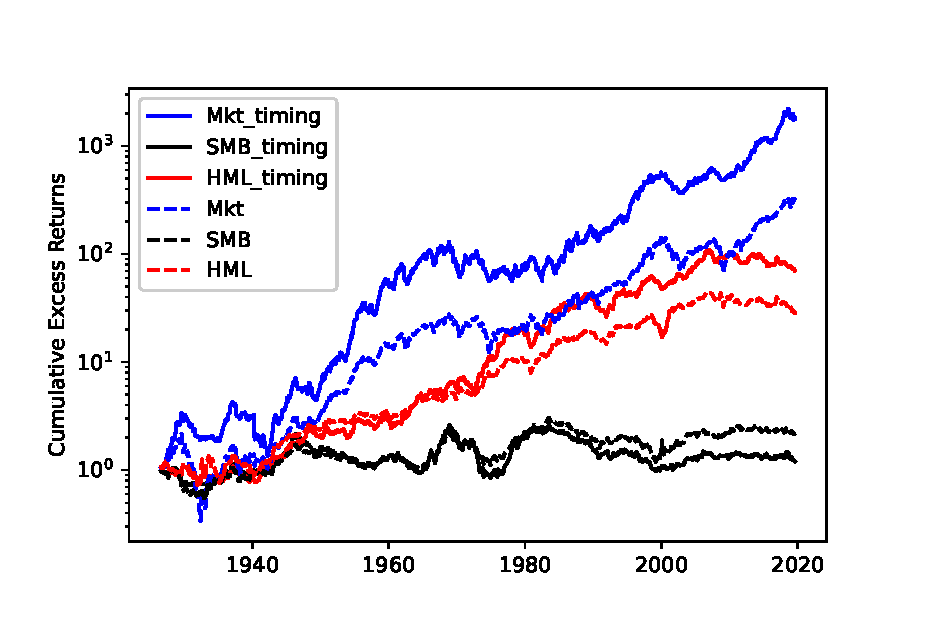
\includegraphics[width=\textwidth]{img/Replication.eps}
			\caption{Cumulative excess returns of buy-and-hold and timing strategy of the three Fama and French factors.}
            \label{fig:replication}
	\end{figure}
	Reference the figure: Figure \ref{fig:replication}. \cite{Busse}
	


	\clearpage\thispagestyle{empty}\addtocounter{page}{-1}\mbox{}
	
	\bibliographystyle{plain}
	\bibliography{references}
	
	
\end{document}
